\chapter{Testy nowej metody}

W tym rozdziale zostaną przedstawione porównania opracowanej metody. W pierwszej kolejności zaprezentowane zostanie zestawienie z metodą wytrenowaną z wykorzystaniem paradygmatu end-to-end, a zatem explicite modelującą ocenę radiologa. Następnie przedstawione zostanie porównanie z wynikami prac algorytmu oceniającego proces gojenia się ścięgna Achillesa z wykorzystaniem danych z Ultrasonografii. Ostatnie zestawienie dotyczyło porównania wyników z oceną biomechaniczną.

Zarówno metoda oparta o paradygmat end-to-end jak i o dane Ultrasonograficzne są wynikiem prac, w których autor tej rozprawy był współautorem i nadzorował grupę studentów opracowujących finalne rozwiązania oraz tworzył plan badań. W przypadku oceny biomechanicznej prace nad metodą zrealizowane zostały w całości przez mgr Magdalenę Syrek z Carolina Medical Center w Warszawie, zatem wartością dodaną tej rozprawy jest przedstawione porównanie.   

\section{Porównanie z metodą opartą o paradygmat end-to-end}

W tej sekcji opracowana metoda zostanie porównana z metodą opartą o paradygmat end-to-end, modelującą explicite ocenę radiologa. Do tego zadania zostały wykorzystane trzy architektury sieci konwolucyjnych opisane w Rozdziale \ref{CNNs} tj. AlexNet, GoogLeNet (Inceptionv3) i ResNet z 50 warstwami konwolucyjnymi (ResNet-50). Wszystkie trzy architektury zostały zmodyfikowane poprzez zastąpienie końcowej warstwy klasyfikacyjnej warstwą regresji z pojedynczym wyjściem i funkcją kosztu zdefiniowaną jako średni błąd kwadratowy. W skutek tego podejścia algorytm szkolony jest, aby minimalizować błąd pomiędzy predykcją sieci neuronowej, a wartościami parametrów z wzorca odniesienia. 

Do szkolenia się sieci wykorzystano powiększony zestaw treningowy, ograniczony jednak do danych z 44 pacjentów treningowych i trzech sekwencji wybranych w toku eksperymentów przedstawionych w podsekcji \ref{seq:protocol_selection}: T2 $^\ast$ GRE, T2 $^\ast$ GRE TE\_MIN i PD. Tym razem nie zdecydowano się na zawężenie zbioru danych tylko do jednej sekwencji RM z uwagi na potrzebę maksymalizację liczebności zbioru. Nie zdecydowano się również na pełny zbiór wszystkich sekwencji, z uwagi na różnice w danych, które mogłyby zaburzać proces szkolenia się end-to-end. 

Do szkolenia zastosowano metodę kroswalidacji z podziałem na 4 segmenty. Dla każdego z parametrów z wzorca odniesienia wyszkolono osobną sieć. Wyliczono metryki MAE, MAX-AE i Corr stosowane również w poprzednim rozdziale. Wyniki zestawiono w Tab. \ref{tab:end-to-endTrain}.
%\vspace{-8px}
\begin{table}[ht]
%\vspace{-px}
\scriptsize
\setlength{\tabcolsep}{1pt}
\centering
\caption{Wyniki szkolenia się sieci w paradygmacie end-to-end z wykorzystaniem zbioru treningowego.}
\label{tab:end-to-endTrain}
\begin{tabular}{lc||c|c|c|c|c|c}
	%\hline
	&& \textbf{SCT} & \textbf{TT} & \textbf{STE} & \textbf{TE} & \textbf{TU} & \textbf{TisE}\\ \hline
	\textbf{AlexNet$_{e}$} & MAE & \textbf{1.04}$\pm$0.33 & \textbf{0.82}$\pm$0.27 & \textbf{0.95}$\pm$0.48 & \textbf{0.88}$\pm$0.38 & \textbf{1.03}$\pm$0.36 & \textbf{0.78}$\pm$0.26  \\
	&MAX-AE & 1.91 & 1.67 & 2.39 & 2.20 & 1.90 & 1.35\\ 
	&Corr & 0.82 & 0.72 & 0.13 & 0.70 & 0.50 & 0.83 \\ \hline
	\textbf{Inceptionv3$_{e}$} & MAE & \textbf{0.88}$\pm$0.32 & \textbf{0.75}$\pm$0.22 & \textbf{0.82}$\pm$0.33 & \textbf{0.78}$\pm$0.20 & \textbf{0.91}$\pm$0.34 & \textbf{0.67}$\pm$0.23 \\
	&MAX-AE & 1.57 & 1.44 & 1.93 & 1.17 & 1.85 & 1.11 \\ 
	&Corr & 0.85 & 0.72 & 0.05 & 0.72 & 0.52 & 0.84 \\ \hline
	\textbf{ResNet-50$_{e}$} & MAE & \textbf{0.64}$\pm$0.21 & \textbf{0.98}$\pm$0.28 & \textbf{0.83}$\pm$0.37 & \textbf{0.89}$\pm$0.22 & \textbf{1.06}$\pm$0.41 & \textbf{1.10}$\pm$0.34  \\
	&MAX-AE & 1.21 & 1.79 & 1.94 & 1.43 & 2.42 & 2.36\\
	&Corr & 0.06 & 0.21 & 0.00 & 0.11 & 0.14 & 0.11\\
	
	
\end{tabular}
%\vspace{-0.5cm}
\end{table}

Otrzymane wartości MAE znajdują się w zakresie 0.64 do 1.10 (w skali wzorca odniesienia 0--7). Dla najlepszego modelu pod względem średniej MAE tj. Inceptionv3, średni dystans między predykcją i wzorcem wyniósł $<0.92$. Najlepiej estymowanymi parametrami były TisE -- 0.67, TT -- 0.75 i TE -- 0.78. Najgorsze rezultaty natomiast otrzymano dla TU -- 0.91, który to parametr silnie zależy od informacji widocznej w płaszczyźnie strzałkowej.

W kolejnej tabeli (Tab. \ref{tab:end-to-end_testset}) przedstawiono zestawienie automatycznej oceny dla zbioru pacjentów testowych, realizowanej przez najlepszy model szkolony w paradygmacie end-to-end (IncepionV3) i proponowaną przez autora tej pracy metodą (SVR).  

\begin{table*}[t]
	\caption{Test set results for the tendon healing progression.}
	\scriptsize
	\begin{center}
		\begin{tabular}{lc||c|c|c|c|c|c}
			\textbf{Model} & & \textbf{SCT} & \textbf{TT} & \textbf{STE} & \textbf{TE} & \textbf{TU} & \textbf{TisE}\\ 
			
\hline
%			AlexNet$_{e}$ &MAE & 1.33$\pm$0.64 & 0.87$\pm$0.11 & $1.38\pm{0.75}$ & 1.16$\pm{0.24}$ & 1.10$\pm{0.27}$& 0.90$\pm{0.19}$ \\
%			& MAX-AE & 2.28 & 1.02 & 2.48 & 1.34 & 1.39 & 1.12 \\ 
%			& Corr & 0.79 & 0.54 & 0.0 & 0.50 & 0.16 & 0.66 \\ \hline
			Inceptionv3$_{e}$ & MAE & 1.12$\pm{0.74}$ & 0.80$\pm{0.24}$ & 1.40$\pm{0.52}$ & \textbf{0.89}$\pm{0.31}$ & 1.08$\pm{0.26}$ & \textbf{0.69}$\pm{0.07}$ \\
			& MAX-AE & 2.14 & \textbf{1.01} & 2.13 & \textbf{1.18} & 1.44 & \textbf{0.78} \\
			& Corr & \textbf{0.82} & \textbf{0.77} & 0.05 & 0.59 & 0.02 & \textbf{0.77} \\ \hline
%			ResNet-50$_{e}$  & MAE & \textbf{0.62}$\pm{0.35}$ & 0.94$\pm0.39$ & 0.94$\pm0.29$ & 1.12$\pm{0.12}$ & 1.08$\pm{0.14}$ & 0.97$\pm{0.43}$ \\
%			& MAX-AE & \textbf{0.93} & 1.52 & \textbf{1.27} & 1.28 & \textbf{1.21} & 1.45 \\
%			& Corr & 0.20 & 0.55 & 0.11 & 0.19 & 0.12 & 0.37\\
%			\hline \hline
			SVR & MAE & $1.05\pm0.12$ & $0.56\pm0.06$ & $0.75\pm0.08$ & $0.91\pm0.10$ & $0.91\pm0.09$ & $0.94\pm0.10$\\
			& MAX-AE & 2.62 & 1.82 & 1.92 & 2.54 & 2.01 & 2.38 \\
			& Corr   & 0.85 & 0.85 & 0.31 & 0.72 & 0.65 & 0.80 
		\end{tabular}
	\end{center}
	\label{tab:end-to-end_testset}
\end{table*}

Metoda SVR osiąga wyższe rezultaty Corr w każdym z parametrów i niższe MAE dla 4 z 6 parametrów. Natomiast tylko w jednym z parametrów (tj. STE) charakteryzuje się niższym MAX-AE. 

Można zatem wnioskować, że cechy wykorzystywane w metodzie SVR do oceny procesu gojenia się skuteczniej dywersyfikują kolejne fazy procesu i pozwalają na ocenę trendu z lepszą dokładnością niż metoda oparta o paradygmat end-to-end. 2 z 6 parametrów, w których pod względem MAE sieć InceptionV3 okazała się lepsza tj. TE i TisE dotyczą obrzęków, zatem elementów ocenianych pod kątem pola powierzchni i kształtu. Fakt ten należy interpretować, iż tego rodzaju informacja dominuje w ekstrahowanych przez jądra splotu obrazach, co z kolei implikuje gorsze wyniki w pozostałych parametrach ocenianych na podstawie wzorców tworzonych przez struktury ścięgniste. Wynik MAX-AE nie jest zaskakujący, ponieważ z uwagi na naturę treningu (explicite modelowanie wzorca odniesienia) maksymalne błędy będą minimalizowane. Trudność w interpretacji polega na fakcie, że maksymalne błędy mogą być wynikiem błędu algorytmu, jak również pojedynczymi omyłkami doświadczonego radiologa, który z uwagi np. na zmęczenie bądź inne dystrakcje zaburzające percepcję, popełnił błąd w ocenie.  

W tym kontekście należy również podkreślić zasadnicze różnice między dwoma przedstawionymi metodami. Do rozwoju metody end-to-end niezbędna jest pełna informacja od radiologa tj. ocena 6 parametrów w kolejnych krokach czasowych. Średnio jest to około 1 godziny pracy na pacjenta. Proponowana przez autora metoda może być dalej rozwijana przy wykorzystaniu danych oznaczonych jako chory, zdrowy oraz znacząco mniejszego zbioru pacjentów z oznaczonym pełnym wzorcem odniesienia, który posłużyłby do sporadycznych ulepszeń etapu meta-regresji. Co prawda metoda wymaga również informacji o ROI, jednakże jest to czas około 10 minut na pacjenta, dla radiologa wykorzystującego odpowiednie oprogramowanie np. Osirix [X] lub VisNow [X]. Ponadto segmentację ROI można stosunkowo łatwo zautomatyzować. Wstępne prace dr. Jędrzeja Nowosielskiego i dr. Piotra Regulskiego oraz autora tej pracy pokazują, że skuteczne w tym zakresie mogą być sieci typu \textit{fully convolutional neural networks}. Przykład działania takiej architektury (tj. U-Net [X]) można zaobserwować na Rys. \ref{fig:segmentacja}. 

\begin{figure}[h]
	\centering
	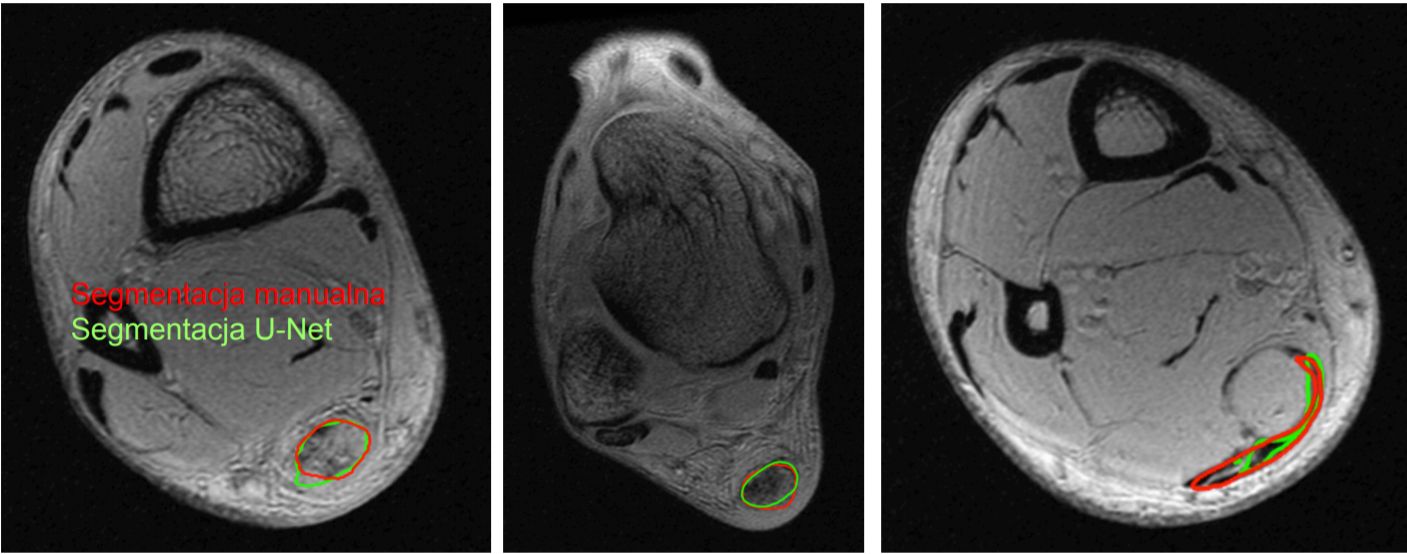
\includegraphics[width=1\textwidth]{figures/Segmentacja.png}
	\caption{Automatyczna segmantacja ROI z wykorzystaniem głębokich sieci neuronowych.}\label{fig:segmentacja}
\end{figure}

Kolorem czerwonym oznaczono obszar segmentacji manulanej, wykonanej przez eksperta radiologa. Kolorem zielonym efekt segmentacji automatycznej. Miara DICE [X] dla otrzymanych obrazów wynosi około 0.75 i świadczy o wysokiej jakości segmentacji oraz o obiecującym kierunku tego rodzaju prac.

Ciekawym elementem rozwoju automatycznej oceny byłaby również fuzja obu metod tj. podmiana ekstraktora cech DL trenowana na binarnie oznaczonym zbiorze na ekstraktor uzyskanego modelu InceptionV3. Jednak z uwagi na omawiane problemy praktyczne z dalszym rozwojem tak utworzonej metody oraz brak obiecujących rezultatów w przeprowadzonych przez autora tej pracy badaniach wstępnych, taka propozycja nie została uwzględniona w prezentowanej rozprawie. 

\section{Porównanie z metodą opartą o dane z ultrasonografii}

W tej sekcji opracowana metoda została porównana z automatyczną oceną bazującą na danych z Ultrasonografii. Ponownie, do utworzenia metody opartej o USG wykorzystano konwolucyjne sieci neuronowe, a dokładniej AlexNet, InceptionV3 i ResNet50 oraz wykorzystano omówiony w poprzedniej sekcji paradygmat end-to-end. 

Dane dla metody opartej o Ultrasonografię pochodziły również z projektu START. Stosowano się zatem do identycznych odstępów czasowych, co w przypadku badań RM i akwizycji poddano tych samych pacjentów. Z przyczyn praktycznych zmniejszyła się jedynie grupa odniesienia, która w tym przypadku wyniosła 18-stu zdrowych ochotników. Badania zrealizowano z wykorzystaniem aparatu GE 3D high-resolution Voluson E8 Expert z liniową sondą (5--18 MHz). Jako dane wejściowe wykorzystano informacje z trybu B (zob. \ref{USG}), których ostateczna liczba wyniosła 565 3D skanów. 

Dane USG są zbliżone do izotropowych dlatego utworzono zbiory zarówno w oparciu o przekroje w płaszczyźnie osiowej jak i strzałkowej (tylko tam, gdzie widoczne jest ścięgno):
\begin{itemize}
	\item zbiór treningowy USG (strzałkowy) -- zawiera 253.639 2D przekrojów w płaszczyźnie strzałkowej, w tym 245.366 pochodzących od chorych 44 pacjentów oznaczonych przez radiologa i 8.273 pochodzących od zdrowych ochotników.
	\item zbiór treningowy USG (osiowy) -- zawiera 467.548 2D przekrojów w płaszczyźnie osiowej, w tym 450.816 pochodzących od chorych 44 pacjentów oznaczonych przez radiologa i 16.732 pochodzących od zdrowych ochotników. 
\end{itemize}

Wizualizacja przykładowych danych USG znajduje się na Rys. \ref{fig:US_sample}.
\begin{figure}[h!]
	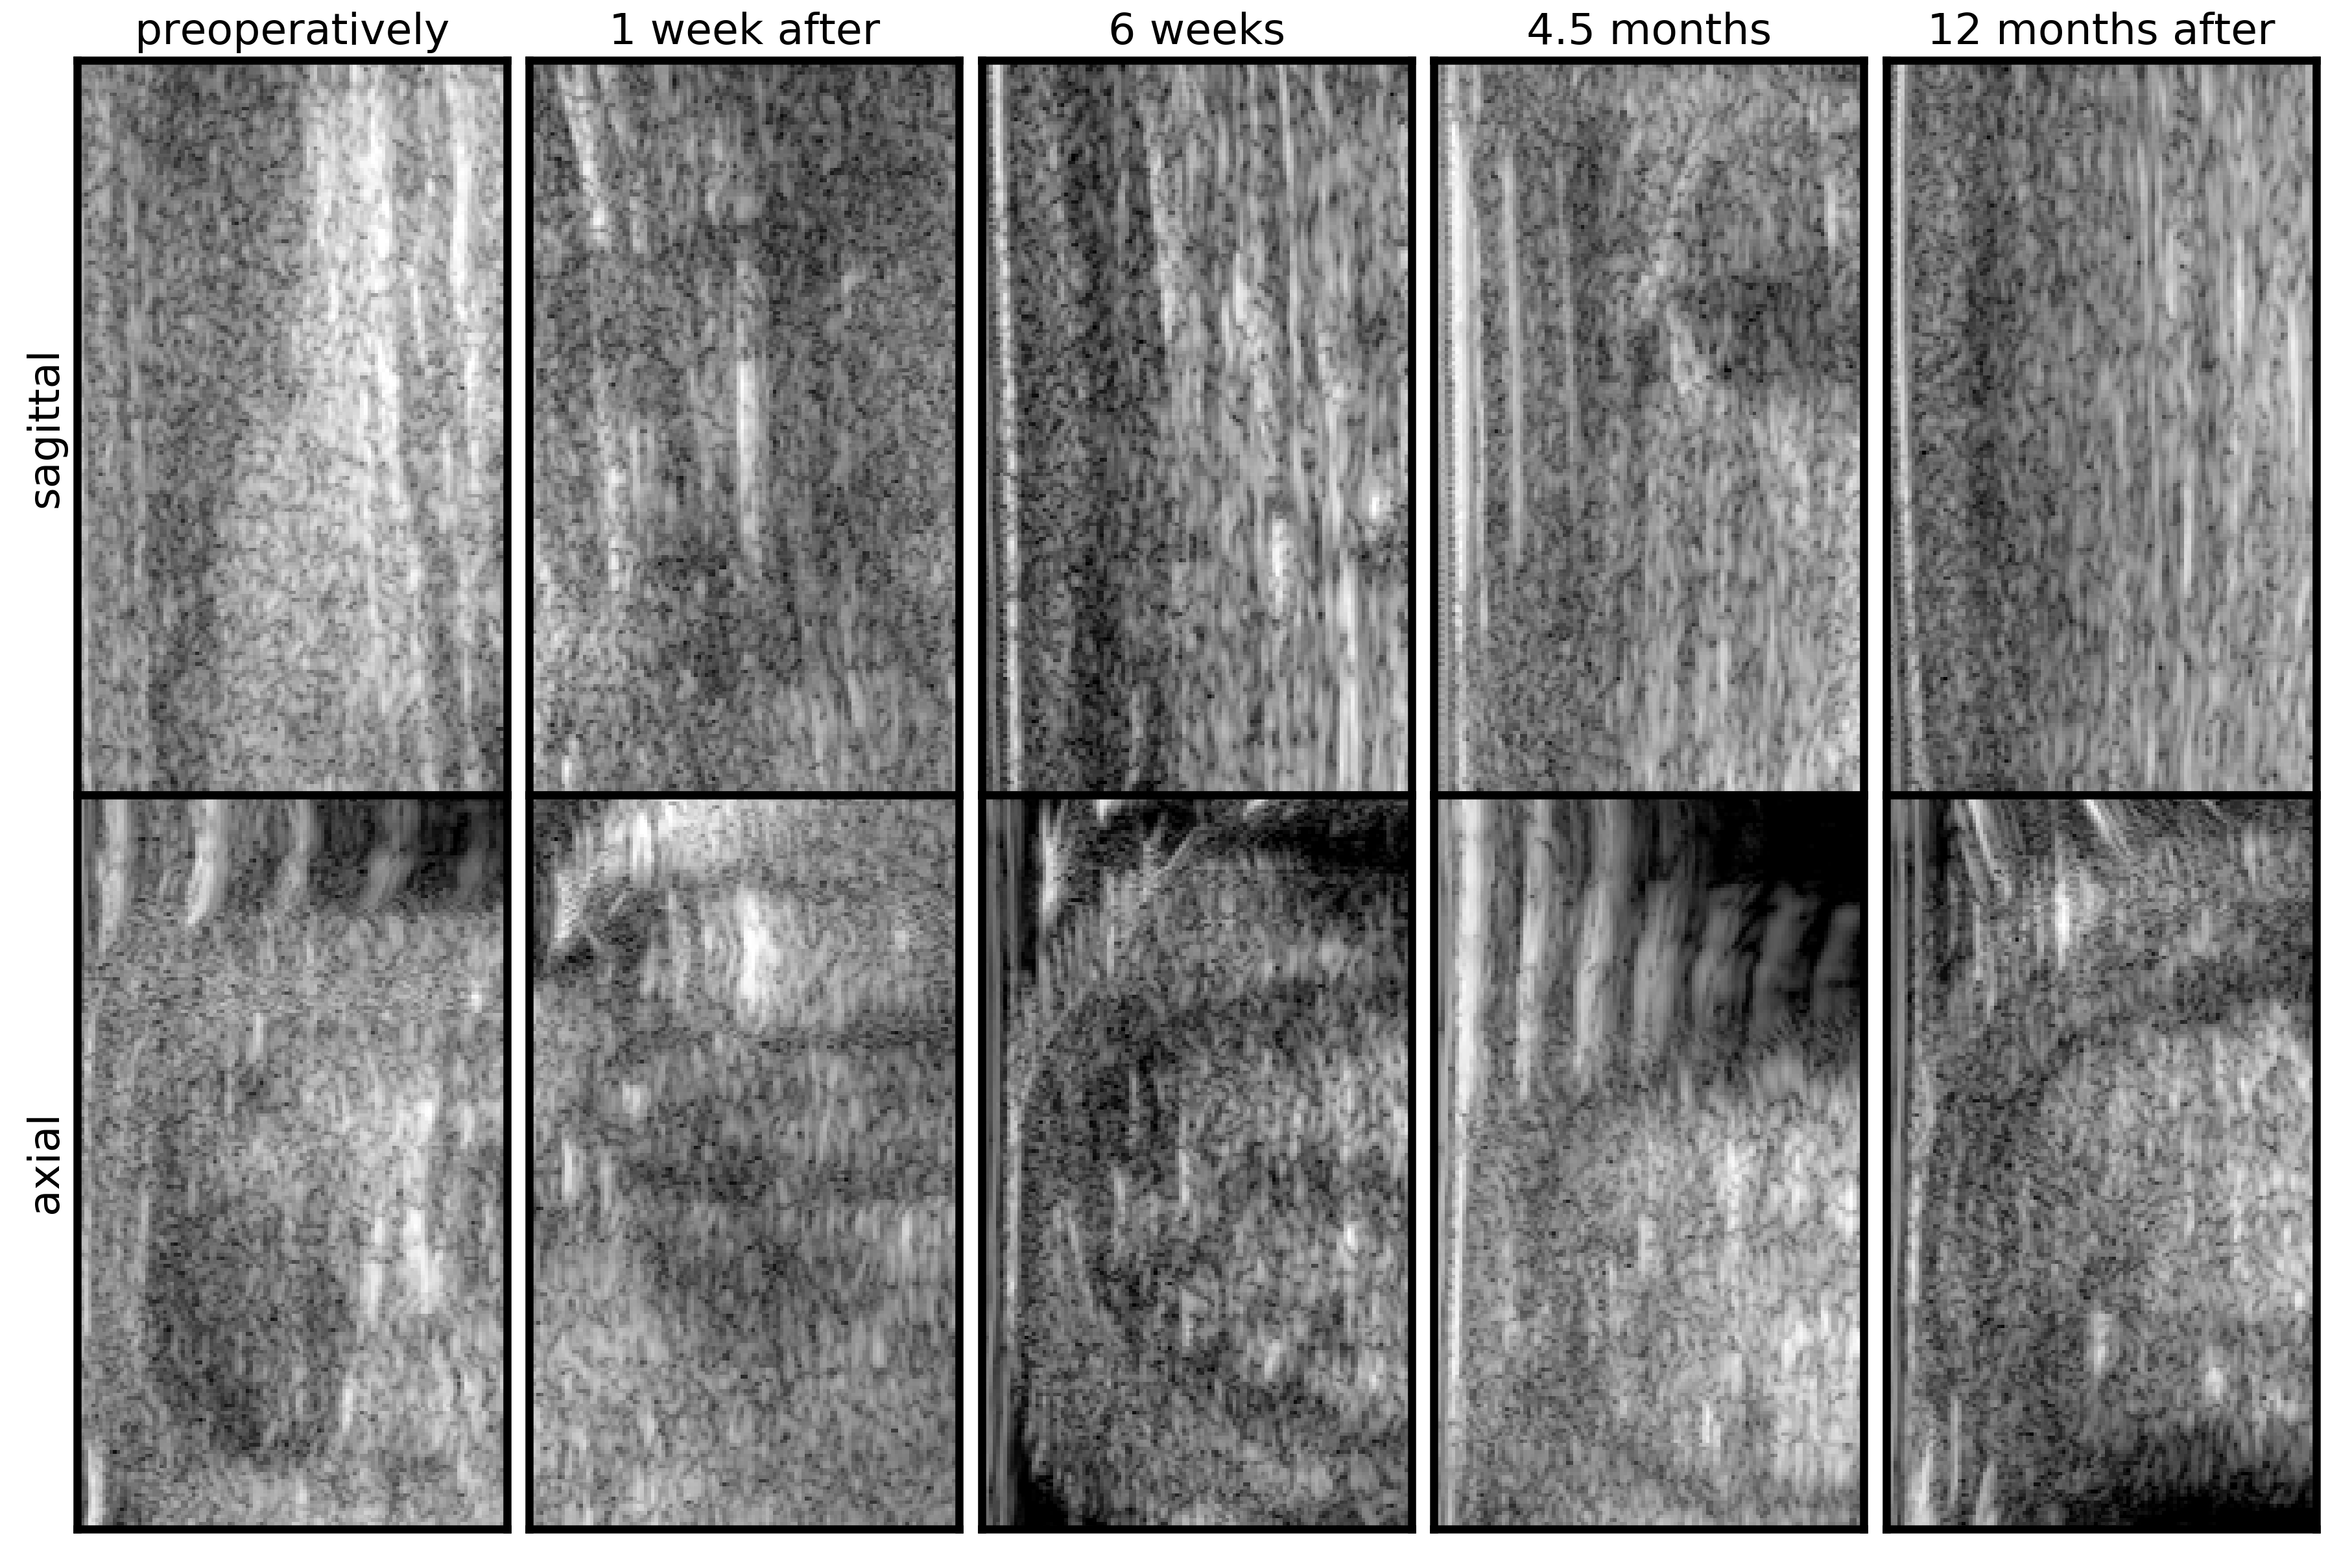
\includegraphics[width=\textwidth]{figures/Data_US_sample.png}
	\caption{Wizualizacja przykładowych danych USG w kolejnych tygodniach po zszyciu ścięgna w przekrojach osiowych i strzałkowych.}
	\label{fig:US_sample}
\end{figure}
W ogólności można zaobserwować ułożenie włókien ścięgnistych na przekrojach strzałkowych i teksturę oraz tkanki otaczające ścięgno na przekrojach osiowych. Jednak szczegółowa analiza załączonych obrazów może być wykonana jedynie przez specjalistę radiologa. 

Utrudniona w stosunku do obrazów RM interpretacja USG ma związek z obecnymi artefaktami w USG i z szumem ziarnistym tworzącym losowe wzorce. Jakość obrazu obniża również jego wartość kliniczną, co wskazują analizy zamieszczone w tej pracy jak i w wielu pracach innych autorów (zob. np. \cite{Khan2003, Ibrahim2013}). Dlatego na początku zdecydowano się przeprowadzić test polegający na prostym zadaniu klasyfikacji binarnej chory/zdrowy (podobnie jak dla badań RM zamieszczonych w Sekcji \ref{binaryMRI}). Ma to na celu porównanie możliwości interpretacji wnioskowania na podstawie obrazów RM i USG. Wyniki dla szkolenia z wykorzystaniem kroswalidacji z 4 segmentami zamieszczono w Tab. \ref{tab:usg-binary}.

\begin{table}[t!]
	\scriptsize
	\centering
	\setlength{\tabcolsep}{3pt}
	\setlength\extrarowheight{2pt}
	\caption{Wyniki szkolenia się sieci na zbiorze treningowym dla danych z USG.}
	\label{tab:usg-binary}
	\begin{tabular}{l||c|c|c||c|c|c}
		%\hline
		& \multicolumn{3}{c}{\footnotesize{\textbf{sagittal}}} & \multicolumn{3}{c}{\footnotesize{\textbf{axial}}} \\
		Architecture & \textbf{Accuracy} & Precision & Recall & \textbf{Accuracy} & Precision & Recall \\ \hline
		AlexNet & 0.846$\pm$00.087 & 0.92$\pm$00.08 & 0.78$\pm$00.11 & 0.843$\pm$00.075 & 0.93$\pm$00.06 & 0.73$\pm$00.11  \\ \hline
		Inception-v3 & \textbf{0.916}$\pm$00.049 & 0.97$\pm$00.04 & 0.90$\pm$00.06 & 0.901$\pm$00.052 & 0.95$\pm$00.3 & 0.87$\pm$00.07 \\ \hline
		ResNet50 & 0.907$\pm$00.039 & 0.96$\pm$00.05 & 0.89$\pm$00.08 & \textbf{0.912}$\pm$00.046 & 0.95$\pm$00.04 & 0.88$\pm$00.06 \\ \hline
	\end{tabular}
\end{table}

Wszystkie modele wyszkolono oddzielnie na przekrojach osiowych i oddzielnie na strzałkowych. Żeby zbalansować dane, przekroje od zdrowych ochotników powiększono poprzez odbicie, a przekroje od chorych pacjentów próbkowano. Dokładność dla najlepszego modelu w przekroju osiowym wyniosła 91.6\%, a w przekroju strzałkowym 91.2\%. Dla porównania, dokładność binarnej klasyfikacji na danych z RM wyniosła 99.83\%. Wyniki te potwierdzają możliwość lepszej interpretacji danych RM dla zadanego problemu, jednak nie dyskryminują USG. W celu polepszenia powyższych rezultatów eksperymentowano również z możliwością klasyfikacji binarnej z wykorzystaniem jedynie obszaru ROI, jednakże działania te przyniosły odwrotny skutek.  

Kolejnym krokiem eksperymentu było porównanie jakości oceny procesu gojenia. W badaniu wykorzystano ponownie paradygmat end-to-end i zmianę warstwy klasyfikującej na regresję z funkcją kosztu określoną jako średni błąd kwadratowy. Dla tej metody próbowano również odtworzyć schemat sprawdzony dla RM, bazujący na treningu binarnym oraz ekstrakcji i redukcji cech, jednak w przypadku USG otrzymane wyniki nie były na tyle satysfakcjonujące, aby zamieszczać je w tej pracy. Ostatecznie wyniki szkolenia sieci w paradygmacie end-to-end zamieszczono w Tab. \ref{tab:usg_train_cross-validation}.

\begin{table}[h]
	\scriptsize
	\setlength{\tabcolsep}{3pt}
	\centering
	\caption{5CV results for the tendon healing progress using end-to-end approach}
	\label{tab:usg_train_cross-validation}
	\begin{tabular}{lc||c|c|c|c|c|c}
		%\hline
		& & \multicolumn{6}{c}{\footnotesize{\textbf{sagittal}}} \\
		\textbf{Network} & & \textbf{SCT} & \textbf{TT} & \textbf{STE} & \textbf{TE} & \textbf{TU} & \textbf{TisE} \\ \hline
		AlexNet & \textbf{MAE} & 0.96$\pm$0.41 & 0.80$\pm$0.27 & 0.82$\pm$0.29 & 0.95$\pm$0.41 & 0.87$\pm$0.39 & 1.08$\pm$0.47  \\
		& MAX-AE & 1.75 & 1.32 & 1.87 & 1.35 & 1.61 & 2.03 \\ 
		& Corr & 0.53$\pm${0.47} & 0.69$\pm${0.38} & 0.11$\pm${0.32} & 0.68$\pm${0.44} & 0.31$\pm${0.51} & 0.22$\pm${0.53} \\ \hline
		Inception-v3 & \textbf{MAE} & \textbf{0.88}$\pm$0.35 & \textbf{0.67}$\pm$0.23 & \textbf{0.80}$\pm$0.31 & \textbf{0.82}$\pm$0.23 & \textbf{0.84}$\pm$0.32 & \textbf{0.93}$\pm$0.29  \\
		& MAX-AE & 1.69 & 1.32 & 1.69 & 1.31 & 1.58 & 1.64 \\ 
		& Corr & 0.83$\pm${0.44} & 0.71$\pm${0.40} & 0.19$\pm${0.34} & 0.64$\pm${0.47} & 0.56$\pm${0.40} & 0.71$\pm${0.40} \\ \hline
		ResNet50 & \textbf{MAE} & \textbf{0.89}$\pm$0.12 & \textbf{0.74}$\pm$0.15 & \textbf{0.83}$\pm$0.22 & \textbf{0.81}$\pm$0.31 & \textbf{0.92}$\pm$0.31 & \textbf{0.99}$\pm$0.32 \\
		& MAX-AE & 1.53 & 1.22 & 1.64 & 1.43 & 1.67 & 1.71 \\
		& Corr & 0.62$\pm${0.31} & 0.38$\pm${0.51} & 0.23$\pm${0.41} & 0.62$\pm${0.51} & 0.12$\pm${0.43} & 0.43$\pm${0.50} \\ \hline \hline
		& & \multicolumn{6}{c}{\footnotesize{\textbf{axial}}} \\
		& & \textbf{SCT} & \textbf{TT} & \textbf{STE} & \textbf{TE} & \textbf{TU} & \textbf{TisE}\\ \hline
		AlexNet & \textbf{MAE} & 0.98$\pm$0.39 & 0.83$\pm$0.33 & 0.82$\pm$0.35 & 0.94$\pm$0.52 & 0.95$\pm$0.50 & 0.86$\pm$0.28  \\
		& MAX-AE & 1.79 & 1.36 & 1.86 & 1.41 & 1.61 & 1.59 \\ 
		& Corr & 0.45$\pm${0.33} & 0.62$\pm${0.39} & 0.20$\pm${0.45} & 0.60$\pm${0.47} & 0.03$\pm${0.42} & 0.59$\pm${0.40} \\ \hline
		Inception-v3 & \textbf{MAE} & \textbf{1.03}$\pm$0.46 & \textbf{0.70}$\pm$0.24 & \textbf{0.76}$\pm$0.26 & \textbf{0.86}$\pm$0.19 & \textbf{0.87}$\pm$0.32 & \textbf{0.85}$\pm$0.25  \\
		& MAX-AE & 2.52 & 1.45 & 1.45 & 1.24 & 1.67 & 1.56 \\ 
		& Corr & 0.77$\pm${0.47} & 0.69$\pm${0.40} & 0.22$\pm${0.37} & 0.65$\pm${0.41} & 0.55$\pm${0.44} & 0.72$\pm${0.41} \\ \hline
		ResNet50 & \textbf{MAE} & \textbf{1.05}$\pm$0.31 & \textbf{0.78}$\pm$0.33 & \textbf{0.80}$\pm$0.24 & \textbf{1.02}$\pm$0.25 & \textbf{0.87}$\pm$0.15 & \textbf{0.91}$\pm$0.28 \\
		& MAX-AE & 1.98 & 1.51 & 1.59 & 1.63 & 1.45 & 1.57 \\
		& Corr & 0.52$\pm${0.41} & 0.47$\pm${0.44} & 0.22$\pm${0.35} & 0.65$\pm${0.55} & 0.18$\pm${0.54} & 0.57$\pm${0.39} \\ \hline \hline
	\end{tabular}
	\vspace{-0.5cm}
\end{table}

Najlepsze rezultaty otrzymano dla sieci Inception-V3 i ResNet-50 dlatego te modele zostały dalej porównane z prezentowaną w tej pracy metodą. W tym celu wyniki MAE, MAX-AE i Corr zostały wyliczone dla zbioru pacjentów testowych i zebrane w Tab. \ref{tab:USGvsRM-cross-validation}.


\begin{table}[h]
	\footnotesize
	\setlength{\tabcolsep}{1pt}
	\centering
	\caption{Porównanie wyników oceny automatycznej bazującej na danych USG i RM na zbiorze testowym.}
	\label{tab:USGvsRM-cross-validation}
	\vspace{-0.5cm}
	\begin{tabular}{lc||c|c|c|c|c|c}
		%\hline
		& & \multicolumn{6}{c}{\normalsize{\textbf{sagittal}}} \\
		\textbf{Network} & & \textbf{SCT} & \textbf{TT} & \textbf{STE} & \textbf{TE} & \textbf{TU} & \textbf{TisE} \\ \hline
%		AlexNet & \textbf{MAE} & 0.90$\pm$0.31 & 0.63$\pm$0.12 & 0.69$\pm$0.31 & 0.81$\pm$0.11 & 0.89$\pm$0.20 & 1.01$\pm$0.35 \\
%		& Corr & 0.55\pm0.15 & 0.70\pm0.24 & 0.22\pm0.49 & 0.61\pm0.28 & 0.12\pm0.43 & 0.28\pm0.27 \\ \hline
		Inception-v3 & \textbf{MAE} & \textbf{0.81}$\pm$0.38 & \textbf{0.63}$\pm$0.06 & \textbf{0.56}$\pm$0.18 & \textbf{0.85}$\pm$0.20 & \textbf{0.54}$\pm$0.04 & \textbf{0.87}$\pm$0.29 \\
		& Corr & 0.80$\pm$0.39 & 0.77$\pm$0.28 & 0.31$\pm$0.33 & 0.52$\pm$0.36 & 0.69$\pm$0.34 & 0.62$\pm$0.52 \\ \hline
		ResNet50 & \textbf{MAE} & \textbf{0.88}$\pm$0.33 & \textbf{0.65}$\pm$0.15 & \textbf{0.66}$\pm$0.09 & \textbf{0.83}$\pm$0.25 & \textbf{0.75}$\pm$0.12 & \textbf{0.93}$\pm$0.22 \\
		& Corr & 0.60$\pm$0.32 & 0.55$\pm$0.38 & 0.25$\pm$0.27 & 0.55$\pm$0.41 & 0.34$\pm$0.29 & 0.56$\pm$0.38 \\
		\hline \hline
		& & \multicolumn{6}{c}{\normalsize{\textbf{axial}}} \\
		& & \textbf{SCT} & \textbf{TT} & \textbf{STE} & \textbf{TE} & \textbf{TU} & \textbf{TisE}\\ \hline
%		\multirow{AlexNet}  & \textbf{MAE} & 1.12$\pm$0.36 & 0.81$\pm$0.29 & 0.58$\pm$0.12 & 0.87$\pm$0.19 & 0.70$\pm$0.24 & 0.85$\pm$0.25 \\
%		& Corr & 0.46$\pm$0.50 & 0.54$\pm$0.32 & 0.26$\pm$0.41 & 0.38$\pm$0.38 & 0.12$\pm$0.34 & 0.70$\pm$0.31 \\ \hline
		Inception-v3 & \textbf{MAE} & \textbf{0.84}$\pm$0.54 & \textbf{0.75}$\pm$1.45 & \textbf{0.58}$\pm$0.10 & \textbf{0.83}$\pm$0.10 & \textbf{0.53}$\pm$0.16 & \textbf{0.83}$\pm$0.30 \\
		& Corr & 0.69$\pm$0.49 & 0.68$\pm$0.41 & 0.45$\pm$0.15 & 0.51$\pm$0.42 & 0.66$\pm$0.16 & 0.68$\pm$0.39 \\ \hline
		ResNet50 & \textbf{MAE} & \textbf{0.92}$\pm$0.37 & \textbf{0.76}$\pm$0.32 & \textbf{0.68}$\pm$0.08 & \textbf{0.81}$\pm$0.17 & \textbf{0.65}$\pm$0.20 & \textbf{0.94}$\pm$0.11 \\
		& Corr & 0.55$\pm$0.41 & 0.57$\pm$0.38 & 0.35$\pm$0.31 & 0.44$\pm$0.39 & 0.39$\pm$0.35 & 0.61$\pm$0.33 \\ \hline \hline
				& & \multicolumn{6}{c}{\normalsize{\textbf{RM}}} \\
		& & \textbf{SCT} & \textbf{TT} & \textbf{STE} & \textbf{TE} & \textbf{TU} & \textbf{TisE}\\ \hline
		SVR & \textbf{MAE} & $1.05\pm0.12$ & $0.56\pm0.06$ & $0.75\pm0.08$ & $0.91\pm0.10$ & $0.91\pm0.09$ & $0.94\pm0.10$\\
		& MAX-AE & 2.62 & 1.82 & 1.92 & 2.54 & 2.01 & 2.38 \\
		& Corr   & 0.85 & 0.85 & 0.31 & 0.72 & 0.65 & 0.80 \\
		\hline \hline
	\end{tabular}
\end{table}

Sieć, uzyskująca najlepsze rezultaty, wytrenowana na USG tj. Inception-v3, uzyskała wartości MAE w zakresie $0.53$ do $0.87$ i uśrednioną korelację Z-Fisher od $0.31$ to $0.80$.
Metoda oparta o USG charakteryzuje się lepszymi rezultatami Corr tylko dla parametrów STE i TU, czyli dla parametrów ocenianych przez wzgląd na krawędzie i na oś w płaszczyźnie strzałkowej. W przypadku miary MAE, metoda RM uzyskuje lepszy rezultat w parametrze TT, gdzie znaczący wpływ na ocenę maja cechy z ROI.

Bazując na powyższych rezultatach można wnioskować, że metoda oparta o dane USG może być komplementarna z proponowaną oceną bazującą na danych z RM. Zwłaszcza w kontekście oceny parametru TU jak i zmniejszenia błędu MAE w poszczególnych parametrach. Do tego celu potrzebna jest jednak dokładna analiza i zrozumienie podstaw wnioskowania sieci opartej o USG, a następnie wybór oraz realizacja odpowiedniej metody fuzji.

\section{Porównanie z metodą opartą o badania biomechaniczne}

W tej sekcji opracowana metoda została porównana z wynikami badań biomechanicznych i funkcjonalnego testu ATRS. Badania te były realizowane w ramach protokołu monitorowania rehabilitacji pacjentów opracowanego w klinice Carolina Medical Center (zob. Sekcja \ref{biomechanika}). 

W ramach projektu START możliwe było zebranie danych dla 30 spośród 60 pacjentów. Dane zawierały wyniki pomiaru zrealizowanego w dwóch krokach czasowych tj. w 26 i 52 tygodniu. Zostały zebrane wyniki ATRS i deficyty sił mięśniowych będące rezultatem badań biomechanicznych. Dokładniej, określono 16 takich deficytów (oznaczonych dalej w tej pracy $d1$--$d16$): w czterech pozycjach tj. kolano zgięte i wyprostowane oraz staw skokowy zgięty wyprostowany zrealizowano pomiary w warunkach izometrii i izokinetyki w trzech prędkościach kątowych 60$^\circ$/s, 120$^\circ$/s oraz 180$^\circ$/s  

Z uwagi na dużą liczbę pomiarów deficytów mięśniowych, w pierwszej kolejność zdecydowano się na przeprowadzenie analizy czynników głównych i identyfikacji nowych zmiennych wyjaśniających w największym stopniu wariancję. Wyniki podsumowano w Tabeli \ref{tab:pca-muscles}.

\begin{table}[t!]
	\scriptsize
	\centering
	\setlength{\tabcolsep}{3pt}
	\setlength\extrarowheight{2pt}
	\caption{Ładunki czynnik.(Brak ) (Input do rownan struktuyralnychNOWE) Wyodrębn. : Składowe główne (Oznaczone ładunki są >,700000).}
	\label{tab:pca-muscles}
	\begin{tabular}{c|c|c|c|c}
		%\hline

		Zmienna&Czynnik1&Czynnik2&Czynnik3&Czynnik4 \\
		\hline
		d1&\textbf{-0,77}&0,16&-0,04&-0,25 \\
		\hline
		d2&0,32&\textbf{-0,74}&0,038&-0,044 \\
		\hline
		d3&\textbf{-0,81}&0,26&-0,17&-0,24 \\
		\hline
		d4&0,09&-0,62&-0,50&-0,38 \\
		\hline
		d5&\textbf{-0,82}&0,13&-0,03&0,21 \\
		\hline
		d6&0,31&-0,53&-0,53&0,42 \\
		\hline
		d7&-0,67&-0,20&-0,34&-0,11 \\
		\hline
		d8&-0,12&-0,34&-0,67&0,43 \\
		\hline
		d9&-0,61&-0,01&-0,28&-0,36 \\
		\hline
		d10&0,07&\textbf{-0,84}&0,26&0,02 \\
		\hline
		d11&\textbf{-0,81}&-0,14&0,01&0,08 \\
		\hline
		d12&-0,11&\textbf{-0,93}&-0,01&-0,01 \\
		\hline
		d13&\textbf{-0,72}&-0,24&0,28&0,36 \\
		\hline
		d14&-0,12&\textbf{-0,81}&0,33&-0,25 \\
		\hline
		d15&-0,58&-0,32&0,39&0,53 \\
		\hline
		d16&-0,17&-0,62&0,23&-0,36 \\
		\hline\hline
		Udział&0,28&0,27&0,10&0,09 \\

	\end{tabular}
\end{table}

Z czterech czynników, 2 mają wyraźnie większy udział w wyjaśnianej wariancji, osiągając odpowiednio poziomy 28 i 27\%. Istotne jest również, że 3 z pięciu znaczących ładunków czynnikowych ($d1$, $d3$, $d5$) dla pierwszego czynnika znajdują się w przedziale $d1$--$d8$, które skojarzone są z pozycją kolana prostego. Dla drugiego czynnika głównego sytuacja jest odwrotna i 3 z czterech ładunków czynnikowych ($d10$, $d12$, $d14$) znajdują się w przedziale $d9$--$d16$, czyli badań przy kolanie zgiętym. Co oczywiste, pozycja kolana wpływa znacząco na wynik badania biomechanicznego. Odzwierciedlają to również rezultaty powyższej analizy. Dlatego w ramach dalszej pracy zdecydowano się na  analizę czynnikową dla wyprostowanego i zgiętego kolana oddzielnie. Wyniki zostały przedstawione w Tabeli \ref{tab:pca-muscles-knee-strait-bended}. 

\begin{table}[t!]
	\scriptsize
	\centering
	\setlength{\tabcolsep}{3pt}
	\setlength\extrarowheight{2pt}
	\caption{Ładunki czynnik.(Brak ) (Input do rownan struktuyralnychNOWE) Wyodrębn. : Składowe główne (Oznaczone ładunki są >,700000).}
	\label{tab:pca-muscles-knee-strait-bended}
	\begin{tabular}{c|c|c||c|c|c}
		%\hline
		
		Zmienna&Czynnik1&Czynnik2&Zmienna&Czynnik1&Czynnik2 \\
		\hline
		d1&\textbf{-0,82}&-0,14&d9&-0,26&0,64 \\
		\hline
		d2&-0,60&-0,37&d10&\textbf{-0,72}&-0,47 \\
		\hline
		d3&\textbf{0,88}&-0,20&d11&-0,52&\textbf{0,73} \\
		\hline
		d4&-0,36&-0,65&d12&\textbf{-0,83}&-0,34 \\
		\hline
		d5&\textbf{0,83}&-0,26&d13&-0,65&0,64 \\
		\hline
		d6&-0,57&-0,64&d14&\textbf{-0,81}&-0,43 \\
		\hline
		d7&0,55&-0,60&d15&-0,67&0,40 \\
		\hline
		d8&-0,03&\textbf{-0,80}&d16&-0,65&-0,38 \\
		\hline\hline
		Udział&0,41&0,26&&0,44&0,27 \\
		
	\end{tabular}
\end{table}

Ponownie można zaobserwować charakterystyczne rozróżnienie, gdzie pierwszy czynnik główny dla badania w pozycji kolana wyprostowanego zawiera ładunki znaczące o nieparzystych numerach, a drugi czynnik posiada znaczące ładunki o parzystych numerach. W przypadku badania w pozycji kolana zgiętego sytuacja jest odwrotna i analogicznie można zaobserwować rozróżnienie. W tym przypadku podział wynika z pozycji stawu skokowego. Ładunki o nieparzystych numerach posiadają czynniki związane z badaniami w zgięciu stawu skokowego, a o parzystych w wyproście. Z uwagi na ten fakt do kolejnych porównań zostały zdefiniowane następujące 4 zmienne:
\begin{enumerate}
	\item $ZZ$ -- wyniki dla pozycji kolano zgięte i staw skokowy zgięty.
	\item $ZW$ -- wyniki dla pozycji kolano zgięte i staw skokowy wyprost.
	\item $WZ$ -- wyniki dla pozycji kolano wyprostowane i staw skokowy zgięty.
	\item $WW$ -- wyniki dla pozycji kolano wyprostowane i staw skokowy wyprostowany.
\end{enumerate} 

Taki podział wydaje się być intuicyjny, ale fakt otrzymania powyższych wyników w analizie numerycznej jest wartością dodaną potwierdzającą spójność danych i jakość przeprowadzonych badań przez fizjoterapeutów z Carolina Medical Center. 

Każda z nowo powstałych zmiennych składa się z czterech pomiarów: jednego dla izometria i trzech dla izokinetyki. Dokładne zestawienie znajduje się w Tabeli [TBD...]

- Tabelka ZZ, ZW, WZ, WW

Ponadto, po stronie danych „fizjoterapeutycznych” jest badanie ATRS .
Badania biomechaniczne i ATRS były wykonane po pół roku i po roku (26 i 52 tydzień) od urazu. 

Na podstawie danych obrazowych oceniono 6 parametrów: 
SCT, STE, TE, TisE, TT, TU
Oceny dokonywano na 2 sposoby: GT (ground truth; doświadczony radiolog) oraz PRED (predykcja za pomocą sieci neuronowych). 
Wykonano analizę czynnikową dla 6 parametrów: osobno dla GT i PRED. 
Wybrano maksymalną liczbę czynników na 2, mimo to program statystyczny zwraca w obu przypadkach 1 czynnik – oznacza to minimalny udział w wyjaśnianej wariancji drugiego czynnika. 

- Tabelka PCA GT
- Tabelka PCA Pred

Jak widać, udział wyjaśnianej wariancji w pierwszym czynniku jest większy dla PRED niż GT – nie jest to zaskakujące, gdyż czynnik ludzki w GT wprowadza nieuniknioną niepewność – wyniki generowane przez człowieka są w pewnym stopniu losowe. 

W następnej części zbadamy korelacje pomiędzy wyżej wymienionymi czynnikami.

-tabelka GTvsPRed

Jak widać wyniki predykcji za pomocą sieci sa silnie skorelowane z ocenami radiologa. To oczywiście bardzo dobrze. 

- Tabelka ATRS vs biomechanika

Widać  korelację  pomiarów wykananych przy takim samym ustawieniu kolana. Co ciekawe, jest to istotniejsze od ustawienia  stawu skokowego (nie wiem czy sformułowanie „ustawienie stawu” jest poprawne). Jak widać ATR słabo koreluje z wynikami pomiarów biomechznicznych . 
Znaki nie są tu istotne, gdyż każda z 4 zmiennyc WW, WZ, ZW, ZZ jest wynikiem analizy czynnikowej. 

- tabelka GT, Pred vs biomechanika i ATRS

Jak widać wskazania radiologa słabo korelują z wynikami badań biomechniacznych oraz ATRS co jest zgodne z praktyką kliniczną – dlatego celowe je1st wykonywanie obu rodzajów badań (radiologicznych i biomechanicznych), gdyż dostarczają innych informacji. 

Jak widać wyniki predykcji za pomocą sieci korelują istotnie z ATRS. Wynik ten jest zapewne spowodowany tym, że wskazania człowieka są obarczone pewną losowością (niemożliwą w zasadzie do uniknięcia). 

\chapter{Podsumowanie}
%- jeden radiolog więc ankieta ok
%- AlexNet uczy się bardziej generycznych cech niż ResNet, który zwraca uwagę na szczególy: https://www.researchgate.net/post/Can_AlexNet_be_a_better_feature_extractor_than_ResNet

%https://icmlviz.github.io/icmlviz2016/assets/papers/4.pdf

%Wydzielenie stanu przed operacją i oznaczenie osobną etykietą w procesie treningu mogłoby doprowadzić do polepszenia rezultatu, co jest sugestią dla przyszłych prac związanych z rozwojem metody.

%TU - Polepszenie w zakresie oceny tego parametru może być uzyskane w przypadku zastosowania bardziej jednorodnych danych RM lub USG.

